\chapter{Relações (3º Bimestre)}

\section{Função exponencial}

\subsection*{Exercício 1 (approximation of e)}

In exercício 4 del 1º bimestre de la 8ª série do Ensino Fundamental,
considered the increasing sequence $u_n = \sum_{k=0}^{n} \frac{1}{k!}$, where
$k! = 1 \times 2 \times \dots \times k$.
We admitted that $u_n$ is convergent and we denoted its limit $e$. We proved
that $e$ não é um racional. In this exercise, we will give an approximation of
$e$:

\begin{enumerate}
\item Calculate $u_6 - \frac{2718}{1000}$
\item For any $n \geq 8$, give an expression of $v_n = (u_n - u_6) \times 7!$
\item Show that $$v_n \leq \sum_{k=0}^{n-7} \frac{1}{8^k} \leq \frac{8}{7}$$
\item Deduce that $2.718 < e < 2.7183$.
\end{enumerate}

\subsection*{Resumo}

For any real number $x$, we admit that the
the sequence $u_n(x) = \sum_{k=0}^{n} \frac{x^k}{k!}$ is convergent and define
%
$$\exp{x} = \lim_{n \rightarrow +\infty} \sum_{k=0}^{n} \frac{x^k}{k!}$$
%
By definition, $\exp{(0)} = 1$ and
$\exp{(1)} = e$ is the Euler number, an irrational
number such that $e \approx 2.718$.
We note that for any reals $x, y$ and natural number $n$:
%
$${u_n(x)} \times {u_n(y)} =
\left(\sum_{p = 0}^{n} \frac{x^p}{p!}\right)
\left(\sum_{q = 0}^{n} \frac{y^q}{q!}\right)
= \sum_{k=0}^{2n} \sum_{p=0}^{k} \frac{x^p}{p!} \frac{y^{k-p}}{{(k-p)}!}
=\sum_{k=0}^{2n} \frac{
\sum_{p=0}^{k} \frac{k!}{{p!}{{(k-p)}!}} x^p y^{k-p}}{k!}
$$
%
We will see in the 3º Bimestre de la 2ª série do Ensino Médio that
the sum in numerator is the expansion of ${(x+y)}^k$.
Hence ${u_n(x)} \times {u_n(y)} = u_{2n}(x+y)$, and taking the limit
when $n \rightarrow +\infty$ we obtain the following property:
%
$$\exp{(x)} \exp{(y)} = \exp{(x+y)}$$
%
In particular, $\exp{(x)} \exp{(-x)} = \exp{(x + {(-x)})} = \exp{(0)} = 1$
and so $\exp{(-x)} = \frac{1}{\exp{(x)}}$.
If $x > 0$ then $\frac{x^0}{0!} = 1$ and for $k \geq 1$ and $\frac{x^k}{k!} > 0$
so $\exp{x} > 1$. If $x < 0$, $\exp{x} = \frac{1}{\exp{|x|}}$ so
$0 < \exp{x} < 1$. If $x > 0$, we actually have
$\exp{x} \geq \frac{x^1}{1!} = x$ and so
$\lim_{x \rightarrow +\infty} e^x = +\infty$.
We deduce that $\lim_{x \rightarrow -\infty} e^x =
\lim_{x \rightarrow -\infty} \frac{1}{e^{|x|}} = 0$.
For $0 \leq x \leq y$ it is easy to see that for all $n$,
$u_n{(x)} \leq u_n{(y)}$ and so $\exp{(x)} \leq \exp{(y)}$, that is $\exp$ is
increasing on $[0, +\infty)$. If $y \leq x \leq 0$, then
$0 \leq {|x|} \leq {|y|}$ so $1 \leq e^{|x|} \leq e^{|x|}$ and
$e^y = \frac{1}{e^{|y|}} \leq \frac{1}{e^{|x|}} = e^x$. So $\exp$ is actually
increasing on $\mathbb R$.

We note that for all natural number $n\geq0$,
%
$$\exp{(n)} = \exp{(
  \underset{n\,\text{times}}{\underbrace{1+1+1+1+1\dots+1}})} =
\underset{n\,\text{times}}{\underbrace{\exp{(1)}\exp{(1)}\dots\exp{(1)}}} = e^n
$$
%
and for any integer $n < 0$, $\exp{n} = \frac{1}{\exp{|n|}} = e^{-|n|} = e^n$.
Now if $p,q$ are two integers
%
$$e^p = \exp{p} = \exp\left(\frac{p}{q} q\right) =
\exp\left(\frac{p}{q}\right)^q$$
%
that is $\exp{\frac{p}{q}} = \sqrt[q]{e^p} = {\sqrt[q]{e}}^p = e^{\frac{p}{q}}$
as defined in 1º bimestre de la 8ª série do Ensino Fundamenta.
Hence $\exp$ generalizes the power of $e$
and we will often just write $\exp{x} = e^x$ for any real $x$.
For any natural number $n$, have formula $e^{n x} =
e^x e^x \dots e^x = {(e^{x})}^n$
($n$ integer and $x$ real). Again, using the definition of power of $e$ from
1º bimestre de la 8ª série do Ensino Fundamenta, we can easily generalize that
to $e^{x y} = {(e^{x})}^y$ for $y$ rational. We will be able to generalize this
to irrational exponents when we define the power to other base than $e$.

If $x < y$ we can find find some large enough integer $n$ such that
$x \leq y - \frac{1}{n} < y$. Then $e^x \leq \frac{e^y}{\sqrt[n]{e}}$
and since $e > 1 \implies \sqrt[n]{e} > 1$ we obtain $e^x < e^y$, that is
$\exp$ is actually strictly increasing. In particular, for any $x,y$
we have $e^x = e^y \iff x = y$. Finally, for any real $x$ and any $h$
such that $|h| < 1$, if $n$ is the largest integer such that
$|h| \leq \frac{1}{n}$ then
$\frac{\exp{(x)}}{\sqrt[n]{e}} = \exp{\left(x - \frac{1}{n}\right)}
\leq \exp{(x+h)}
\leq \exp{\left(x + \frac{1}{n}\right)} = \exp{(x)} \sqrt[n]{e}$.
So using the fact that $\lim_{n \rightarrow +\infty} \sqrt[n]{e} = 1$ we deduce that
$\exp{(x+h)}$ has limit $\exp{(x)}$ when $h$ tends to $0$
that is the graph of $\exp$ in
a cartesian coordinate system is a continous curve as shown
in red in the following schema. We note that $\exp$ grows faster than
any power function $x \mapsto x^n$ (see Exercise 10).

\begin{center}
  \begin{tikzpicture}
    \draw[->] (-3.5,0) -- (3.5,0) node[right] {$x$};
    \draw[->] (0,0) -- (0,9) node[above] {$y$};
    \draw[color=red, domain=-2:2] plot (\x,{2.718^\x}) node[left] {$y=\exp(x)$};
    \draw[color=green, domain=-1:3] plot (\x,{\x}) node[left] {$y=x$};
    \draw[color=blue, domain=-2.5:2.5] plot (\x,{\x * \x}) node[left] {$y=x^2$};
    \draw(-2,0)node[below]{$-1$};
    \draw(-1,0)node[below]{$-1$};
    \draw(0,0)node[below]{$0$};
    \draw(1,0)node[below]{$1$};
    \draw(2,0)node[below]{$2$};
    \draw(0,1)node[left]{$1$};
    \draw(0,3)node[left]{$3$};
    \draw(0,5)node[left]{$5$};
    \draw(0,7)node[left]{$7$};
  \end{tikzpicture}
\end{center}

\subsection*{Exercício 2}

Simplify the following expressions:

\begin{enumerate}
\item $\exp{(-3)} \times \exp{(7)}$
\item $\frac{\exp{6}}{\exp{5}}$
\item $\exp{(4-2^2)}$
\item $\frac{\exp{8}}{\exp{(-2)}}$
\item $\lim_{x \rightarrow +\infty} \exp{(-x^2)}$
\item $\lim_{x \rightarrow +\infty} \frac{\exp{(4x)}}{\exp{(2x)}}$
\item $\sup_{x \in \mathbb R} \exp{(-x^2+12x-31)}$
\item ${(\exp{2})}^3$
\item $\sqrt[3]{\exp{54}}$
\item $\lim_{x \rightarrow 5} \exp{(3x - 8)}$
\end{enumerate}

\subsection*{Exercício 3}

Find the solutions of the following equations:

\begin{enumerate}
\item $e^{x} - e^3 = 0$
\item $e^{x} + e^3 = 0$
\item $e^{3x+5} - e^{26} = 0$
\item $e^{3x^2 - 15x} + e^{-\frac{75}{4}} = 0$
\item $e^{3x^2 - 15x} - e^{-\frac{75}{4}} = 0$
\item $e^{x^2} - \frac{e^{21}}{e^{4x}} = 0$
\item $-e^{9x} + e^{3x^2+7}= 0$
\item $e^{2x} + 7 e^x + 1 = 0$
\item $e^{2x} - 2 e^x + 1 = 0$
\item $2 e^{x+3} - e^4 + 5e^{x+1} + e^{2x} = 3e^{2x} + e^4 + 3e^{x+1}$
  (set $X = e^x$).
\item $e^{x+3} - 8 e^{x-2} = -8 e^3 + e^{2x-2}$ (set $X = e^x$).
\item $e^{-5} + 3e^{-x-5} = e^{-x-3} + 3e^{-2x-3}$ (set $X = e^x$).
\item $3e^{4x} + 7e^{2x} = 9 e^{3x}$ (set $X = e^x$).
\item $e^{2x+5} + 2e^{5-x} = e^{5x} + 2e^{2x}$ (set $X = e^{3x}$).
\item $e^{2x^2 - 3x} + 11e^{x^2 - 2x} = 11 e^{6-x} + e^{x^2 - 2x + 6}$
  (set $X = e^{x^2-x}$)
\end{enumerate}

\subsection*{Exercício 4}

Solve the following inequations:

\begin{enumerate}
\item $e^{3x-1} \leq e^{4x+2}$
\item $5e^{9x-2} + 7e^x \geq 11e^{5x-1}$ (set $X = e^{4x-1}$).
\item $e^{2x+5} + e^{2x-3} \leq e^2 + e^{4x}$ (set $X = e^{2x}$).
\item $e^{7x} + 10e^{4x} \geq e^{4x+6} - e^{4x} + 11 e^{x+6}$ (set $X = e^{3x}$).
\item $2e^{25} - e^{2x^2 -8x+8}
  \leq  2e^{x^2-4x+4} -  e^{x^2-4x+29}$ (set $X = e^{{(x-2)}^2}$).
\end{enumerate}

\section{Função logarítmica}

\subsection*{Resumo}

For any $y > 0$, there is a unique real $x$ such that $\exp{x} = e^x = y$.
We note $x = \ln{(y)}$ and call it the natural logarithm.
By definition for all $x$,
$\ln e^x = x$ and for all $y > 0$, $\ln e^y = y$.
We have $e^0 = 1$ and so $\ln{1} = 0$.
For any $y > 0$, we have $\frac{1}{y} > 0$. If $x = \ln{y}$ then $e^{x} = y$.
Then $e^{-x} = \frac{1}{y}$ and so
${\ln\left(\frac{1}{y}\right)} = -x = -\ln{y}$.
If $y_1, y_2 > 0$ then $e^{\ln{(y_1)} + \ln{(y_2)}} =
e^{\ln{(y_1)}} e^{\ln{(y_2)}}
= y_1y_2$ and so $\ln{(y_1y_2)} = \ln{(y_1)} + \ln{(y_2)}$.
For any rational $q$ and $y > 0$, we have $y^q > 0$.
We also have $ e^{q \ln{(y)}} = {\left(e^{\ln{(y)}}\right)}^q = y^q$ and so
$\ln{(y^q)} = q \ln{(x)}$. Again, this will later be generalized to nonrational
exponents.

Given any point $A=(a,b)$ in a cartesian coordinate system, let $B=(b,a)$ and
$(D)$ is the metriatriz of $[PQ]$. By definition, $A$ is the symmetric of $B$
with respect to $(D)$. For any $x$, the point $P=(x,x)$ verifies
$AP = BP = \sqrt{{(a-x)}^2+{(b-x)}^2}$ and so $P \in (D)$. So actually $(D)$
is the line of equation $y = x$. Let
$G_{\exp} = {\{ {(x,e^x)} : x \in {\mathbb R} \}}$
be the graph of $\exp$. The symmetric of $G_{\exp}$ with respect to $(D)$ is
${\{ {(e^x,x)} : x \in {\mathbb R} \}}$. But
${\{ e^x : x \in {\mathbb R} \}} = {\{ y : y > 0 \}}$
and for any $y > 0$, $x=\ln{y}$ is the unique real such that $y = e^x$.
So the symmetric of $G_{\exp}$ with respect to $(D)$ is actually
${\{ {(y,\ln{y})} : y > 0 \}} = G_{\ln}$, the graph of $\ln$. We can do the same
reasoning for other function and its inverse function, for example
for any integer $n$, $G_{x \geq 0 \mapsto x^n}$ and $G_{x \geq 0 \mapsto \sqrt[n]{x}}$
are symmetric
with respect to $(D)$. We can now extend our previous schema to draw
$y=\ln(x)$. By symmetry, we deduce properties of $\ln$ from those of $\exp$:
it is
continuous, strictly increasing, $\lim_{n \rightarrow 0^+} \ln{(x)} = -\infty$
and $\lim_{n \rightarrow +\infty} \ln{(x)} = +\infty$.
Also, $\ln$ grows slower than
any root function $x \mapsto \sqrt[n]{x}$ (see Exercise 10).

\begin{center}
  \begin{tikzpicture}
    \draw[->] (-2,0) -- (9,0) node[right] {$x$};
    \draw[->] (0,-2) -- (0,9) node[above] {$y$};
    \draw[color=red, domain=-2:2] plot (\x,{2.718^\x}) node[left] {$y=\exp(x)$};
    \draw[color=green, domain=-2:5] plot (\x,{\x}) node[left] {$(D) \; y=x$};
    \draw[color=blue, domain=-2.5:2.5] plot (\x,{\x * \x}) node[left] {$y=x^2$};
    \draw[color=blue, domain=0:2.5] plot ({\x * \x},\x) node[above] {$y=\sqrt{x}$};
    \draw[color=red, domain=-2:2] plot ({2.718^\x}, \x) node[above] {$y=\ln(x)$};
    \draw(1,0)node[below]{$1$};
    \draw(3,0)node[below]{$3$};
    \draw(5,0)node[below]{$5$};
    \draw(7,0)node[below]{$7$};
    \draw(0,1)node[left]{$1$};
    \draw(0,3)node[left]{$3$};
    \draw(0,5)node[left]{$5$};
    \draw(0,7)node[left]{$7$};
  \end{tikzpicture}
\end{center}

\subsection*{Exercício 5}

Simplify the following expressions:

\begin{enumerate}
\item $\ln{(256)}$
\item $\ln{({(x-1)(x+2)} - x^2 + 3 - x)}$
\item $\ln{(4e^2)}$
\item $\left(e^{\frac{\ln{(7)}}{3}}\right)^{9}$
\item $\ln{\frac{27}{e^4}}$
\item $\lim_{x \rightarrow 0} \ln{\left({(5+x)}^2+3{|x|}\right)}$
\item $\lim_{x \rightarrow \infty} \ln\left(\frac{6}{1+x^2} + \frac{7}{x}\right)$
\item $\inf_{x \in \mathbb R} {\ln(3x^2+30x+91)}$
\end{enumerate}

\subsection*{Exercício 6}

Find the solutions of the following equations:

\begin{enumerate}
\item $e^{27x} - 11 = 0$
\item $\ln{(3x+2)} + 15 = 0$ (where $x > -\frac{2}{3}$)
\item $63e^{3x} + 2e^{4x} = e^{5x}$
\item $e^{3x} - \ln{(2)} e^{2x} + e^{2x} = 4e^{2x} - 3 \ln{(2)} e^x$
\item $e^{x^2+2x-1} - \ln{(a)}e^{x^2+x-1} + 11e^{x^2+x-1}+8\ln{(a)}e^{x^2-1} =
  -3\ln{(a)}e^{x^2-1}$ for any constant $a > 0$.
\item $3{\ln{(x)}}^2 + 4e^6{\ln{(x)}}
  - \ln{(2)}\ln{(x)}  = 2\ln{(2)}\ln{(x)} + 3\ln{(2)} e^6 + e^6{\ln{(x)}}$
  (where $x > 0$)
\item $3 \times \ln{(3x^2 -12x + e^8 + 12)} = 24$
\item $e^{17x} = \ln{\left(a^2-3a+3\right)}$ for any constant $a$.
\end{enumerate}

\subsection*{Exercício 7}

Solve the following inequations:

\begin{enumerate}
\item $e^{x+9} \leq 17$
\item $\ln{(x-7)} \geq 11$ (where $x > 7$)
\item $e^{2x} - e^{x} \geq 2e^{x} + 88$
\item $e^{3x} + 41e^x \leq 20 e^{2x} -50e^x$
\item $\ln{(x-2)}^2 +8\ln{(x-2)} \geq 26 - 3\ln{(x-2)}$ (where $x > 2$)
\end{enumerate}

\section{Generalization}

\subsection*{Resumo}

For any $b > 0$ we define
$\exp_b{(x)} = \exp{(x \ln{(b)})}$. We note that for any rational $q$,
$\exp_{b}{(q)} = \exp{(q \ln{(b)})} = {(e^{\ln{(b)}})}^q = b^q$. So $\exp_b$ is
a generalization of the power of $b$ for irrational exponents and we will
just write $\exp_b{(x)} = b^x$. By definition, we have
%
$$\ln{y^x} = x \ln{(y)}$$
%
for any $x$ and $y > 0$.
Also, by definition we have for all $x,y$:
%
$${\left(e^{x}\right)}^y = e^{y \ln{(e^x)}} = e^{xy}$$
$${\left(b^{x}\right)}^y = e^{y \ln{(x^b)}} = e^{y \ln{(e^{x \ln{b}})}} =
e^{xy \ln{b}} = b^{xy}$$
%
We easily other similar properties as what we found for $\exp$:

\begin{enumerate}
\item $\exp_b{0} = 1$ and $\exp_b{1} = b$
\item For any $x$, $\exp_b{(x)} > 0$.
\item For any $x,y$, $\exp_b{(x+y)} = \exp_b{(x)} \exp_b{(y)}$
\item For any $x$, $\exp_b{(-x)} = \frac{1}{\exp_b{(x)}}$
\item
  If $b = 1$, then $\exp_b$ is the constant function $x \mapsto 1^x = 1$.
  If $b > 1$, $\exp_b$ is strictly increasing
  $\lim_{x \rightarrow -\infty} \exp_b{x} = 0$ and
  $\lim_{x \rightarrow +\infty} \exp_b{x} = +\infty$.
  If $0 < b < 1$, $\exp_b$ is strictly decreasing
  $\lim_{x \rightarrow -\infty} \exp_b{x} = +\infty$ and
  $\lim_{x \rightarrow +\infty} \exp_b{x} = 0$.
\item $\exp_b$ is a continuous function.
\item If $b \neq 1$ then for all $x,y$, we have
  $\exp_b{(x)} = \exp_b{(y)} \iff x = y$
\end{enumerate}

If $b > 0$ and $b \neq 1$, we can define $\log_b{y}$ as the unique $y$ such that
$b^x = y$. We call it the logarithm in base $b$.
Again, we have similar properties as $\ln$:

\begin{enumerate}
\item $\log_b{1} = 0$ and $\log_b{b} = 1$
\item For any $y > 0$, $\log_b{(y)} \leq 0$ if $y \leq 1$ and.
  $\log_b{(y)} \geq 0$ if $y \geq 1$.
\item For any $x,y > 0$, $\log_b{xy} = \log_b{(x)} + \log_b{(y)}$
\item For any $y > 0$, $\log_b{\frac{1}{y}} = -\log_b{y}$
\item If $b > 1$, $\log_b$ is strictly increasing
  $\lim_{y \rightarrow 0} \log_b{y} = -\infty$ and
  $\lim_{y \rightarrow +\infty} \log_b{y} = +\infty$.
  If $0 < b < 1$, $\log_b$ is strictly decreasing
  $\lim_{y \rightarrow +\infty} \exp_b{x} = -\infty$ and
  $\lim_{x \rightarrow 0} \exp_b{x} = +\infty$.
\item $\log_b$ is a continuous function.
\item For all $x,y > 0$, $\log_b{(x)} = \log_b{(y)} \iff x = y$
\item For all $y > 0$ and $x$, $\log_b{y^x} = x \log_b{(y)}$
\end{enumerate}

Let $b_1, b_2 > 0$ be two bases such that $b_1,b_2\neq0$.
For any $y > 0$, we set $x = \log_{b_1}{(y)}$.
Then $y = b_1^x = \left(b_2{^{\log_{b_2}{(b_1)}}}\right)^x =
b_2^{x \log_{b_2}{(b_1)}}$. We conclude that
$\log_{b_2}{(y)} = x \log_{b_2}{(b_1)}$. Since $b_1 \neq 1$,
$\log_{b_2}{(b_1)} \neq 0$ and so
$\log_{b_1}{(y)} = \frac{\log_{b_2}{(y)}}{\log_{b_2}{(b_1)}}$. In particular for
any base $b$, we can express its logarithm as
%
$$\log_{b}{(y)} = \frac{\ln{(y)}}{\ln{(b)}}$$
%
So $\log_b$ is just $\ln$ multiplied by a scalar.

\subsection*{Exercício 8}

\begin{enumerate}
\item For any natural number $k$, how many digits do we need to write $10^k$
  in base 10?
\item For any natural number $n$, how many digits do we need to write $n$
  in base 10?
\item How many digits do we need to write an integer $n$ in base $2$ and $16$?
\item Express $\log_{16}$ in function of $\log_{2}$
\item Write $15$ and $5$ in base $2$ and $16$.
\item Write $229$ in base $2$ and $16$. What do you notice?
  Is it consistent with the previous questions?
\end{enumerate}

\subsection*{Exercício 9}

Place the values below on a rule using the following logarithm scale:
$d$ meters are placed at coordinate $x = \log_{10} d$. What is the advantage of
using such a logarithm scale?

\begin{enumerate}
\item Diameter of Phosphorus atom: $1\text{Å} = 10^{-10}\text{m}$.
\item Diameter of red blood cell: 7 micrometers.
\item Forelius pusillus Ant: 1mm.
\item Human height: 1.75m.
\item Height of Cristo Redentor: 38m.
\item Distance from São Paulo to Rio de Janeiro: 358km.
\item Earth circumference: 40000km.
\item Distance Earth-Moon: 400000km.
\item Distance Sun-Earth: 150 millions of kilometers.
\item Distance of Proxima Centauri from the Earth: 4.22 Light-years.
  (1 Light-year is about $9.4607 \times 10^{15} \text{m}$)
\end{enumerate}

\subsection*{Exercício 10 (difficult)}

\begin{enumerate}
  \item Show that for all natural number $n \geq 0$, we have $2^n > n$.
  \item Pick an arbitrary natural number $k > 0$.
    Verify that for any $n \geq k+1$ we have
    $\frac{2^n}{n} = 2^{k+1}
    \frac{2^{n-k-1}}{n-k-1} \left(1-\frac{k+1}{n}\right)$.
  \item Deduce that for $n \geq 2{(k+1)}$ we have
    $\frac{2^n}{n} \geq 2^k > k$.
  \item Deduce that $\lim_{x \rightarrow +\infty} \frac{2^x}{x} = +\infty$.
  \item We now fix a real number $\alpha > 0$. For any $b > 0$
    and $x > 0$ simplify the expression
    $$
    \frac{1}{b^\alpha} \left( \frac{\left(e^{\frac{b}{\alpha}}\right)^{\frac{x}{b}}}{\frac{x}{b}} \right)^\alpha
    $$
  \item Explain why we can find $b > 0$ such that
    $e^{\frac{b}{\alpha}} \geq 2$.

  \item Conclude that
    $\lim_{x \rightarrow +\infty} \frac{e^x}{x^\alpha} = +\infty$.

  \item Let $K > 0$. Explain why we can find $x > 1$ such that
    $\frac{e^x}{x^{\frac{K}{\alpha}}} > 1$.
    Show that $y = x^{1/\alpha}$ satisfies
    $\frac{y^{\alpha}}{\ln{(y)}} > K$.
  \item We admit that $y \mapsto \frac{y^{\alpha}}{\ln{(y)}}$ is increasing
  on $[e^{1/\alpha}, +\infty)$.
    Deduce the value of
    ${\lim_{y \rightarrow +\infty} \frac{y^\alpha}{\ln{(y)}}}$.

\end{enumerate}

\section{Solução do Exercícios}

\subsection*{Exercício 1 (approximation of e)}

\begin{enumerate}
\item After simplification, we find $u_6 - \frac{2718}{1000} = \frac{1}{18000}$
\item We find $v_n = 1 + \frac{1}{8} + \frac{1}{8 \times 9} +
  \frac{1}{8 \times 9 \times 10} + ... + \frac{1}{8 \times 9 \times \dots
    \times n}$.
\item Clearly, for any $8 \leq k \leq n$
  $8 \times 9 \times \dots \times k \geq 8^{k - 7} > 0$ and so
  $\frac{1}{8 \times 9 \times \dots \times k} < \frac{1}{8^{k-7}}$.
  Hence
  $$v_n \leq 1 + \sum_{k = 8}^{n} \frac{1}{8^{k-7}} =
  \sum_{k = 0}^{n-7} \frac{1}{8^k}$$
  We recognize the sum of a geometric series of factor $\frac{1}{8}$ and so
  $v_n \leq \frac{1}{1 - \frac{1}{8}} = \frac{8}{7}$
\item We have $e \geq u_6 = 2.178 + \frac{1}{18000} > 2.71805$.
  and $e = \lim_{n\rightarrow +\infty} u_n \leq
  \lim_{n\rightarrow +\infty} {(\frac{v_n}{7!} + u_6)} \leq
  2.718 + \frac{1}{18000} + \frac{8}{7 \times 7!} <
  2.7183$
\end{enumerate}

\subsection*{Exercício 2}

\begin{enumerate}
\item $e^{7-3} = e^4$
\item $e^{6-5} = e$
\item $e^0 = 1$
\item $e^{8-{(-2)}} = e^{10}$
\item $0$ (because $\lim_{x \rightarrow +\infty} -x^2 = -\infty$)
\item $\lim_{x \rightarrow +\infty} e^{2x} = +\infty$ (because
  $\lim_{x \rightarrow +\infty} 2x = +\infty$)
\item The maximum of $x \mapsto -x^2+12x-31$ is $5$ (obtained at $x=6$).
  Since $\exp$ is increasing the
  $\sup_{x \in \mathbb R} \exp{(-x^2+12x-31)} = e^5$.
\item ${(\exp{2})}^3 = \exp{2 \times 3} = e^6$
\item $\sqrt[3]{\exp{54}} = \exp{\frac{54}{3}} = e^{18}$
\item By continuity of $\exp$,
  $\lim_{x \rightarrow 5} \exp{(3x - 8)} = e^{3 \times 5 - 8} = e^7$
\end{enumerate}

\subsection*{Exercício 3}

\begin{enumerate}
\item $e^{x} = e^3$ iff $x = 3$
\item This would imply $e^{x} = -e^3 < 0$ so there is no solution.
\item $e^{3x+5} = e^{26}$ iff $3x+5=26$ iff $x = 7$.
\item This would imply $e^{3x^2 - 15x} = -e^{-\frac{75}{4}} < 0$
  so there is no solution.
\item $e^{3x^2 - 15x} - e^{-\frac{75}{4}} = 0$ iff
  $e^{3x^2 - 15x} = e^{-\frac{75}{4}}$ iff
  $3x^2 - 15x + \frac{75}{4} = 0$ iff $x = \frac{5}{2}$.
\item $e^{x^2} - \frac{e^{21}}{e^{4x}} = 0$ iff
  $e^{x^2} = e^{21-4x}$ iff $x^2 + 4x - 21 = 0$ iff $x=3$ or $x = -7$.
\item $-e^{9x} + e^{3x^2+7}= 0$ iff $e^{3x^2+7} =e^{9x}$
  iff $3x^2 - 9x + 7 = 0$. The discriminant of this equation is
  strictly negative so there is no solution.
\item $e^{2x}, e^x > 0$ so $e^{2x} + 7 e^x + 1 > 0$ and there is no solution.
\item $e^{2x} - 2 e^x + 1 = 0$
  iff ${(e^x - 1)}^2 = 0$ iff $e^x = 1$ iff $x = 0$.
\item $2 e^{x+3} - e^4 + 5e^{x+1} + e^{2x} = 3e^{2x} + e^4 + 3e^{x+1}$ iff
  $2 e^{x+3} + 2e^{x+1} -2e^{2x} - 2e^4 = 0$ iff
  $e^{x+3} + e^{x+1} -e^{2x} - e^4 = 0$. If we let $X = e^x$ we this equivalent
  to $-X^2 + {(e^3 + e)} X - e^4 = 0$. The discriminant of this equation
  is $\Delta = {(e^3+e)}^2 - 4 e^4 = e^6 + 2e^4 + e^2 - 4e^4 =
  e^6 - 2e^4 + e^2 = {(e^3-e)}^2$. Since $e^3 > e$ we have
  $\sqrt{\Delta} = e^3 - e$ and the equation in $X$ has two solutions:
  $X_1 = \frac{-e^3-e-{(e^3 - e)}}{-2} = e^3$ and
  $X_2 = \frac{-e^3-e+{(e^3 - e)}}{-2} = e$.
  Finally, the equation in $x$ has two solutions: $x = 3$ (if $e^x = X = X_1$)
  and $x=1$ (if $e^x = X = X_2$).
\item $e^{x+3} - 8 e^{x-2} = -8 e^3 + e^{2x-2}$ iff
  $-X^2 e^{-2} + {(e^3 - 8 e^{-2})} X + 8e^3 = 0$.
  The discriminant of the equation
  is $\Delta = {(e^3-8e^{-2})}^2 + 32 e =
  e^6 -16e + 64e^{-4} + 32e = e^6 +16e + 64e^{-4} = {(e^3+8e^{-2})}^2$
  and since $e^3+8e^{-2} > 0$ we have $\sqrt{\Delta} = e^3+8e^{-2}$.
  Hence the solution of the equation in $X$ are
  $X_1 = \frac{-e^3 + 8 e^{-2} + e^3+8e^{-2}}{-2e^{-2}} = -8 < 0$
  and $X_2 = \frac{-e^3 + 8 e^{-2} - e^3-8e^{-2}}{-2e^{-2}} = e^{5}$.
  $e^x > 0$ so $e^x = X_1$ is impossible. So the only solution is given
  by $e^x = X_2 = e^{5}$ that is $x = 5$.

\item $e^{-5} + 3e^{-x-5} = e^{-x-3} + 3e^{-2x-3}$ iff
  $e^{-5} + \frac{3e^{-5}}{X} - \frac{e^{-3}}{X} - \frac{3e^{-3}}{X^2} = 0$.
  Since $X = e^x > 0$ this is equivalent to
  $X^2 + {(3 - e^{-2})}X - 3e^2 = 0$.
  As above, we find two solutions $X_1 = -3$ and $X_2 = e^2$ for $X$ so there is
  only one solution $x = 2$.
\item
  As above, we obtain the equivalent equation
  $3X^2 -9X + 7$ which has a strictly negative
  discriminant. Hence the original equation does not have any solution.

\item By setting $X = e^{3x}$,
  this is equivalent to
  $X^2 + (2-e^5)X - 2e^5$, which has only on positive solution $X = e^5$.
  Hence the unique solution is $x = \frac{5}{3}$.

\item By setting $X = e^{x^2-x}$ this is equivalent to
  $X^2 + {(11 - e^6)}X - 11e^6$. This equation has only one positive solution
  $X = e^6$. So the original equation is equivalent to $x^2 - x = 6$
  which has exactly two solutions $x = 3$ and $x = -2$.

\end{enumerate}

\subsection*{Exercício 4}

\begin{enumerate}
\item Since $\exp$ is increasing, $e^{3x-1} \leq e^{4x+2}$ iff
  $3x - 1 \leq 4x +2$ iff $x \geq -3$.
\item By setting $X = e^{4x-1}$, this is equivalent to
  $5X^2 -11X + 7 \geq 0$. The discriminant of $5X^2 -11X + 7$ is
  $\Delta = 11^2 - 4 \times 5 \times 7 = -19 < 0$ so
  $5X^2 -11X + 7 \geq 0$ is true for any $X$. Hence the original inequality
  is true for any $x$.
\item By setting $X = e^{2x}$, this is equivalent to
  $X^2 -{(e^5 +e^{-3})} X + e^2 \geq 0$. This polynomial has two roots
  $e^{-3}$ and $e^5$, so it is $\geq 0$ iff $X \leq e^{-3}$ or $X \geq e^{5}$.
  So the original inequation is true iff $x \leq \frac{-3}{2}$ or
  $x \geq \frac{5}{2}$.
\item By setting $X = e^{3x}$, this is equivalent to
  $X^2 - {(e^6-11)}X - 11e^6 \geq 0$.
  This polynomial has two roots
  $e^{6}$ and $-11$, so it is $\geq 0$ iff
  $X \leq -11$ or $X \geq e^{6}$. Since $X = e^{3x} > 0$ the original
  inequality holds iff $X \geq e^{6}$ iff $x \geq 2$.
\item By setting $X = e^{{(x-2)}^2}$,
  this is equivalent to
  $X^2 - {(e^{25} - 2)} X - 2e^{25} \geq 0$. The polynomial has two roots
  $X_1 = -2$ and $X_2=e^{25}$ and it is $\geq 0$ iff
  $X \leq -2$ or $X \geq e^{25}$. Since $X = e^{{(x-2)}^2} > 0$
  the original inequality holds iff $(x-2)^2 \geq 25$ iff
  $x \leq -3$ or $x \geq 7$.

\end{enumerate}

\subsection*{Exercício 5}

\begin{enumerate}
\item $\ln{(2^{8})} = 8 \ln{(2)}$
\item $\ln{(1)} = 0$
\item $2{(\ln{(2)}) + 1}$
\item $343$
\item $3\ln{(3)} - 4$
\item Using the continuity of $\ln$, we obtain $2\ln{(5)}$
\item $-\infty$ (the limit of the expression inside $\ln$ is $0$)
\item $x \mapsto 3x^2+30x+91$ reaches its minimum $16$ at $x=-5$. Since
  $\ln$ is increasing, $\inf_{x \in \mathbb R} {\ln(3x^2+30x+91)} =
  \ln{16} = 4\ln{(2)}$.
\end{enumerate}

\subsection*{Exercício 6}

\begin{enumerate}
\item $x = \frac{\ln{(11)}}{27}$
\item $x = \frac{e^{-15} - 2}{3}$
\item If we set $X = e^{x} > 0$ this is equivalent to $X^2 -2X - 63 = 0$.
  The equation in $X$ has two solutions: $X=9$ or $X=-7$. So the equation
  in $x$ has only one solution: $x = \ln{(9)} = 2\ln{(3)}$
\item If we set $X = e^{x} > 0$ this is equivalent to
  $X^2 - {(\ln{2} + 3)}X + 3 \ln{(2)} = 0$.
  The equation in $X$ has two solutions: $X=3$ or $X=\ln{2} > 0$.
  So the equation
  in $x$ has only two solutions: $x = \ln{(\ln{(2)})}$ and $X=\ln{(3)}$
\item If we let $X = e^{x} > 0$ this is equivalent to
  $X^2 + {(\ln{a} + 11)}X + 11 \ln{(a)} = 0$.
  The equation in $X$ has two solutions: $X=-11 < 0$ or $X=-\ln{a}$.
  If $a \geq 1$ then $-\ln{a} \leq 0$ so there is no solution.
  If $0 < a < 1$ then $-\ln{a} > 0$ so there is one solution
  $x = \ln{(\ln{(a)})}$.
\item If we set $X = \ln{(x)}$ for all $x > 0$, then this is equivalent to
  $X^2 - {(\ln{(2)}-e^6)} X -\ln{(2)}e^6$. The equation in $X$ has two
  solutions: $X = \ln{(2)}$ and $X = -e^6$.
  So the equation in $x$ has two solutions:
  $x = 2$ and $x = e^{-{e^6}}$.
\item This is equivalent to $3x^2 - 12x + 12 = 0$ that is
  $x = 2$.
\item If $a \in [1,2]$ then $a^2-3a+3 \leq 1$ and so
  $\ln{\left(a^2-3a+3\right)} < 0$ and there is no solution.
  If $a < 1$ or $a > 2$,
  there is one solution $x = \frac{\ln{(\ln{\left(a^2-3a+3\right)})}}{17}$.
\end{enumerate}

\subsection*{Exercício 7}

\begin{enumerate}
\item $x \leq \ln{(17)} - 9$
\item $x \geq e^{11} + 7$
\item If $X = e^x$ this is equivalent to
  $X^2 -3X - 88 \geq 0$ and this polynomial has two roots: $X = 11$ and $X=-8$.
  So the solution is $x \geq \ln{(11)}$.
\item If $X = e^x$ this is equivalent to
  $X^2 -20X + 91 \leq 0$ and this polynomial has two roots: $X = 7$ and $X=13$.
  So the solution is $\ln{7} \leq x \leq \ln{13}$.
\item If $X = \ln{(x-2)}$ then this is equivalent to
  $X^2 +11X - 26 \geq 0$. The inequation in $X$ is satisfied iff
  $X \geq 2$ or $X \leq -13$, so the inequation in $x$ is satisfied iff
  $x \geq e^2 + 2$ or $2 < x \leq e^{-13} + 2$.
\end{enumerate}

\subsection*{Exercício 8}

\begin{enumerate}
\item If $10^k = \underset{k\,\text{zeros}}{\underbrace{1000\dots000}}$
  so we need $k+1$ digits.
\item If we note $k = \left\lfloor \log_{10}{(n)} \right\rfloor$
  the integer part of $\log_{10}{(n)}$ we have
  $k \leq \log_{10}{(n)} < k+1$ and so
  $10^k \leq n < 10^{k+1}$. Hence we need exactly $k+1$ digits.
\item Similarly, we get $\left\lfloor \log_2{(n)} \right\rfloor$ and
  $\left\lfloor \log_{16}{(n)} \right\rfloor$.
\item For all $x > 0$,
  we have $\log_{16}(x) = \frac{\log_2{x}}{\log_2{16}} = \frac{\log_2{x}}{4}$

\item $15$ written ``E'' in base $16$ and ``1110'' in base $2$ ;
  $5$ is ``5'' in base $16$ and ``101'' in base $2$.

\item $229$ is written ``E5'' in base $16$ and ``11100101'' in base $2$.
  We note that we can obtain the former from the latter by grouping
  consecutive 0's and 1's into block of $4$ digits
  (``1110'' and ``0101'') and then by writing each of this block in base $16$
  (``E'' and ``5''). So we approximately need $4$ times less digits in base
  $16$ than in base $2$, which is consistent with the previous questions.

\end{enumerate}

\subsection*{Exercício 9}

\begin{center}
  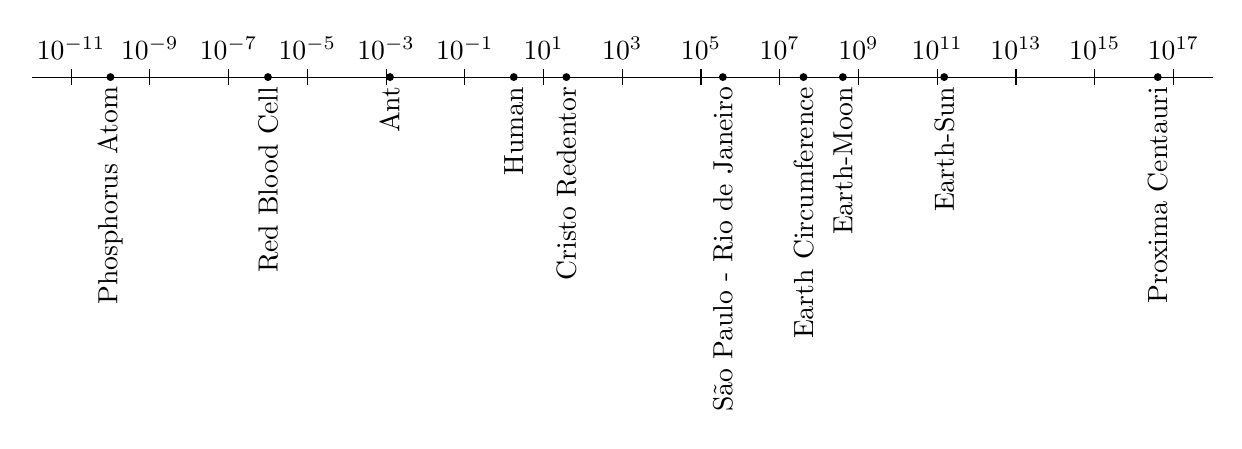
\begin{tikzpicture}
    \draw (-6,0) -- (9,0);
    \foreach \x in {-11,-9,-7,-5,-3,-1,1,3,5,7,9,11,13,15,17}
      \draw (\x/2,-.1) --(\x/2,.1) node[above] {$10^{\x}$};

      \fill (-5,0) circle(.05)
      node[rotate=90, left]{Phosphorus Atom};

      \fill (-3,0) circle(.05)
      node[rotate=90, left]{Red Blood Cell};

      \fill (-1.45,0) circle(.05)
      node[rotate=90, left]{Ant};

      \fill (0.1215190243431472,0) circle(.05)
      node[rotate=90, left]{Human};

      \fill (0.789891798308405,0) circle(.05)
      node[rotate=90, left]{Cristo Redentor};

      \fill (2.776941513321937,0) circle(.05)
      node[rotate=90, left]{São Paulo - Rio de Janeiro};

      \fill (3.801029995663981,0) circle(.05)
      node[rotate=90, left]{Earth Circumference};

      \fill (4.30102999566398,0) circle(.05)
      node[rotate=90, left]{Earth-Moon};

      \fill (5.58804562952784,0) circle(.05)
      node[rotate=90, left]{Earth-Sun};

      \fill (8.300617861064941,0) circle(.05)
      node[rotate=90, left]{Proxima Centauri};
  \end{tikzpicture}
\end{center}

We note that the logarithm scale allows to represent infinitely small and
infinitely large values on the same schema.

\subsection*{Exercício 10 (difficult)}

\begin{enumerate}
\item
  For $n = 0$, $2^0 = 1 > 0$.
  For $n = 1$, $2^1 = 2 > 0$. More generally, for $n \geq 1$ if
  $2^{n} > n$ then we also have $2^{n+1} = 2 \times 2^n > 2 \times n = n + n \geq
  n + 1$ and so the property is also true for $n+1$. Hence the property is true
  for all $n$.
  Alternative proof:
  $1 < 2 < 2^1 < 2^2 < \dots < 2^{n-1}$ are $n$ distinct integers
  $< 2^n$ and so $n < 2^n$.

\item We have $\frac{2^n}{n} = \frac{2^{k+1} 2^{n-k-1}}{n} =
  2^{k+1} \frac{2^{n-k-1}}{n-k-1} \frac{n-k-1}{n}$ from which we get the desired
  equality.
\item If $n \geq 2{(k+1)}$ then
  $\left(1-\frac{k+1}{n}\right) \geq \frac{1}{2}$. By the first question,
  we also have $\frac{2^{n-k-1}}{n-k-1} > 1$. By the previous question we get
  $\frac{2^n}{n} > 2^k$. By the first question again, we deduce
  $\frac{2^n}{n} > k$.

\item By the previous question,
  $\lim_{n \rightarrow +\infty} \frac{2^n}{n} = +\infty$
  If $n$ is the integer part of $x$ then
  $n > x - 1$ and
  $\frac{2^x}{x} \geq \frac{2^n}{n+1} = \frac{2^n}{n} \frac{n}{n+1}$.
  When $x$ tends to $+\infty$, then so does $n$
  and so $\frac{2^n}{n} \frac{n}{n+1}$ tends to $+\infty$. Hence
  $\lim_{x \rightarrow +\infty} \frac{2^x}{x} = +\infty$.

  \item Using the property of the power, we find
    $$
    \frac{1}{b^\alpha} \left( \frac{\left(e^{\frac{b}{\alpha}}\right)^{\frac{x}{b}}}{\frac{x}{b}} \right)^\alpha =
    \frac{e^{\left(\frac{b}{\alpha} \frac{x}{b} \alpha \right)}}{b^\alpha \frac{x^\alpha}{b^\alpha}} = \frac{e^x}{x^\alpha}
    $$

  \item $e > 1$ and $\alpha > 0$ so $e^{\frac{1}{\alpha}} > 1$ and so
    $\lim_{x \rightarrow +\infty} \left(e^{\frac{1}{\alpha}}\right)^x = +\infty$.
    In particular for some $b$ large enough we have
    $e^{\frac{b}{\alpha}} = \left(e^{\frac{1}{\alpha}}\right)^b \geq 2$.

  \item We pick $b$ such that $2 \leq e^{\frac{b}{\alpha}}$ and consider
    $x > 0$. Then $\frac{x}{b} > 0$ and
    so $0 < \frac{2^{\left(\frac{x}{b}\right)}}{\frac{x}{b}} \leq
    \frac{\left(e^{\frac{b}{\alpha}}\right)^{\frac{x}{\alpha}}}{\frac{x}{b}}$.
    We have $\lim_{x \rightarrow +\infty} \frac{2^{\left(\frac{x}{b}\right)}}{\frac{x}{b}} = +\infty$ and since $\alpha > 0$, we deduce that
%%
    $$
    {\lim_{x \rightarrow +\infty}
      \frac{e^x}{x^\alpha}} =
    {\lim_{x \rightarrow +\infty} \frac{1}{b^\alpha} \left( \frac{\left(e^{\frac{b}{\alpha}}\right)^{\frac{x}{b}}}{\frac{x}{b}} \right)^\alpha}
 = +\infty
    $$

  \item This is just because
    $\lim_{x\rightarrow +\infty} \frac{e^x}{x^{K/\alpha}} = +\infty$ by
    the previous question (with $\alpha$ replaced with $K/\alpha$).
    From $1 < \frac{e^x}{x^{K/\alpha}}$
    we get $0 < x^{K/\alpha} < e^x$ and taking the logarithm
    $K \ln{(x^{1/\alpha})} < x$ and so $K < \frac{x}{\ln{(x^{1/\alpha})}}$
    since we assumed $x > 1$.
    Now if $y = x^{1/\alpha}$, this becomes
    $\frac{y^\alpha}{\ln{(y)}} > K$.

  \item We showed that $\frac{y^\alpha}{\ln{(y)}}$ can be made larger than any
    constant $K$. If we admit that $y\mapsto \frac{y^\alpha}{\ln{(y)}}$
    is increasing for large enough values then this means
    ${\lim_{y \rightarrow +\infty} \frac{y^\alpha}{\ln{(y)}}} = +\infty$.
    Note that the hypothesis is necessary:
    ${(K+1)} \cos{(2\pi \times K)} = K+1 > K$ but
    $y \mapsto {(y+1) \cos{(2\pi \times y)}}$ ``oscillates'' above and below
    0 and so does not have any limit at $+\infty$.

\end{enumerate}
